% Phụ lục tiếng Việt (đã gọt) cho mainvi.tex. Giữ nguyên số liệu/nhãn/hình/tên model.
% Các phần thất bại/bị loại được dồn thành một đoạn ngắn; kết quả đạt chất lượng giữ đầy đủ.
\section{Phần mở rộng phân đoạn (đăng ký trước)}
\label{app:segmentation}
Phần mở rộng này được đăng ký trước sau khi đã xem các quan sát GPU lịch sử; nó không đăng ký hồi tố cho chúng. Nó hỏi liệu việc dựng mask theo từng đối tượng, chứ không phải NMS, có tạo ra chi phí mỗi-đối-tượng lớn hơn không. Các phép đo thiết bị và đếm tấn công dùng 20 ảnh đầu (xếp theo thứ tự từ điển) của COCO128-seg, không phải một cohort held-out độc lập. Trọng số pretrained và mọi định danh ảnh được ràng buộc bằng manifest SHA-256. Dùng nhiễu toàn ảnh dạng số; không đánh giá patch vật lý ở đây.

\subsection{Khối lượng mask tổng hợp và chất lượng đo}
YOLOv8n-seg được đánh giá ở FP32, $640\times640$, confidence 0.25 và IoU 0.45. NMS dùng một kernel torchvision cố định. Forward và NMS trên ảnh thật được nối tiếp bởi các hệ số mask và hộp tiêm tất định ở $K\in\{0,10,50,100,300\}$. Thời gian toàn trình được đo trực tiếp; thời gian mask cũng được đo riêng. Tùy chọn độ phân giải proto dùng \texttt{upsample=False}, như trong micro-benchmark lịch sử, và không được trình bày như bộ dự đoán triển khai mặc định. Mask toàn độ phân giải dùng \texttt{process\_mask\_native}. Mỗi ảnh có năm lần lặp, thứ tự điều kiện ngẫu nhiên hóa, hai bản sao A/A ở $K=0$, và một tham chiếu forward ảnh cố định trước mỗi ảnh. Bộ đếm thời gian GPU đồng bộ ở cả hai biên. Affinity CPU được đọc lại và kiểm chứng dưới tải. Host thuê báo tên i7-12700K nhưng để lộ 18 logical processor đồng nhất; không suy ra được danh tính P/E-core hay lõi vật lý. Điều kiện CPU dưới đây ghim logical processor 2--5 với bốn intra-op thread. Tỷ số lấy $K=10$ làm cơ sở, trung vị theo ảnh rồi trung bình hình học; khoảng tin cậy lấy mẫu lại 20.000 lần với seed 20261106. MDE là xấp xỉ $t$ trung tâm công suất 80\% trên log tỷ số A/A. $K^*$ là $K>10$ nhỏ nhất có cận dưới của tỷ số vượt $\exp(\mathrm{MDE}_{\log})$.
\begin{table*}[t]\centering
\caption{Khối lượng mask tổng hợp (đăng ký trước). Tỷ số là thời gian toàn trình đo trực tiếp ở $K=300$ so với $K=10$, có điều kiện trên cohort cố định. Chỉ gồm các lần chạy đạt cổng chất lượng đã đăng ký.}
\label{tab:seg-device}
\begin{adjustbox}{max width=\textwidth}\begin{tabular}{llrrrr}\toprule
Thiết bị & Dựng mask & Tỷ số toàn trình [95\% CI] & MDE (\%) & $K^*$ & Số cờ trôi\\\midrule
CPU, 4 logical processor & Độ phân giải proto & 1.091 [1.076, 1.107] & 2.07 & 300 & 0 \\
CPU, 4 logical processor & Toàn độ phân giải & 3.951 [3.914, 3.996] & 1.61 & 50 & 0 \\
RTX 5060 Ti & Độ phân giải proto & 1.046 [1.032, 1.060] & 1.38 & 300 & 2 \\
RTX 5060 Ti & Toàn độ phân giải & 1.926 [1.919, 1.934] & 1.88 & 50 & 2 \\
\bottomrule\end{tabular}\end{adjustbox}\end{table*}
\begin{figure*}[t]\centering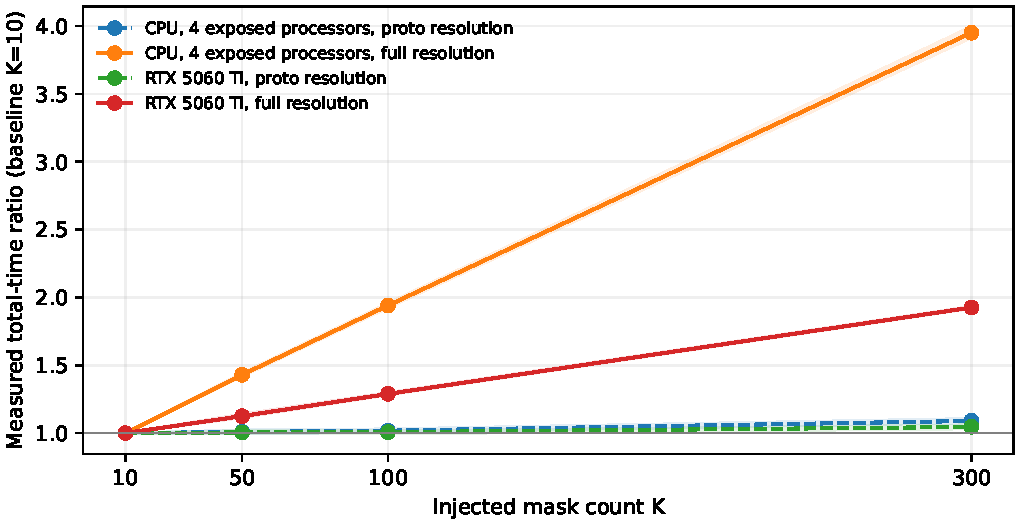
\includegraphics[width=0.85\textwidth]{segmentation_extension/mask_dose_response.pdf}\caption{Dose-response khối lượng mask tổng hợp trên hai lần chạy thiết bị đạt chất lượng. Vùng bóng là khoảng bootstrap-ảnh 95\%; tỷ số so với $K=10$.}\label{fig:seg-dose}\end{figure*}
Lần chạy CPU-4-processor có 0 điểm tham chiếu bị cờ và cả hai kiểm tải đạt; lần GPU có hai điểm bị cờ, trong mức tối đa cho phép là hai. Một lần chạy CPU đơn-processor riêng có mười điểm bị cờ và bị loại khỏi bảng này. Các lần laptop trước vẫn bị loại. Các đối chứng tổng hợp này thiết lập một mặt chi phí, không phải hiệu quả tấn công.

\subsection{Nhiễu thật và chuyển sang mô hình không NMS (YOLO26)}
Xác nhận tấn công đón đầu tái dùng mục tiêu PGD toàn ảnh lịch sử và ngân sách cố định ($L_\infty=16/255$, 100 bước, bước $2/255$). Nó đánh giá iterate cuối, không phải iterate tốt nhất trên quỹ đạo. Trên YOLOv8n-seg, trung vị số giữ lại đổi từ 2.5 lên 270; 20/20 ảnh đạt $K\ge100$ và 6/20 đạt cap 300. CÙNG các nhiễu đó được chuyển sang YOLO26n-seg với head một-một bật tường minh ($\texttt{end2end=True}$). Số đếm lấy trực tiếp từ cột confidence 4 của đầu ra native $[1,300,38]$ ở ngưỡng 0.25, không áp NMS. Trung vị mục tiêu đổi từ 2 lên 3; 0/20 ảnh đạt $K\ge50$. Vậy thí nghiệm này không tái lập chuyển số-đếm-cao sang đường native không NMS. Nó không thiết lập miễn nhiễm với một tấn công đặc thù mục tiêu. Các quan sát YOLO26 số-đếm-cao trước đó dùng đường suy luận/đếm khác và không hỗ trợ một tuyên bố native không NMS.

\subsection{Mở rộng sang cohort xác nhận 500 ảnh rời}
Sau các quan sát COCO128, một nghiên cứu đón đầu riêng khóa 500 trong 5.000 ảnh COCO val2017 chính thức bằng lấy mẫu đều không hoàn lại (seed 20261106). Các ảnh này rời khỏi cohort 20 ảnh trước đó. Ngân sách và quy tắc iterate-cuối không đổi; đánh giá FP32 dùng batch size 4 cố định trước. Kernel theo batch có thể khác số học so với thực thi batch-một. Mỗi mô hình nguồn tối ưu nhiễu riêng; mục tiêu YOLO26 nhận cùng nhiễu tối ưu trên YOLOv8n. Các cohort báo cáo riêng, không gộp.
\begin{table*}[t]\centering\caption{Nghiên cứu đếm COCO-val500 mới. Khoảng cho trung vị lấy mẫu lại ảnh 20.000 lần; khoảng tỷ lệ dùng cận Wilson 95\%. Ngưỡng chung $K=50$ là endpoint đếm, không phải ngưỡng độ trễ đã hiệu chuẩn cho mọi mô hình.}\label{tab:seg-val500}
\begin{adjustbox}{max width=\textwidth}\begin{tabular}{lrrlr}\toprule Mô hình/đường & Ảnh & Trung vị $K$ sạch & Trung vị $K$ nhiễu [95\% CI] & Số $K\ge50$ [95\% tỷ lệ CI]\\\midrule
YOLOv8n-seg & 500 & 4 & 300 [300, 300] & 500/500 [99.24\%, 100.00\%] \\
YOLO11n-seg & 500 & 3 & 300 [300, 300] & 500/500 [99.24\%, 100.00\%] \\
YOLO26 native, chuyển & 500 & 3 & 3 [3, 4] & 0/500 [0.00\%, 0.76\%] \\
\bottomrule\end{tabular}\end{adjustbox}\end{table*}
\begin{figure*}[t]\centering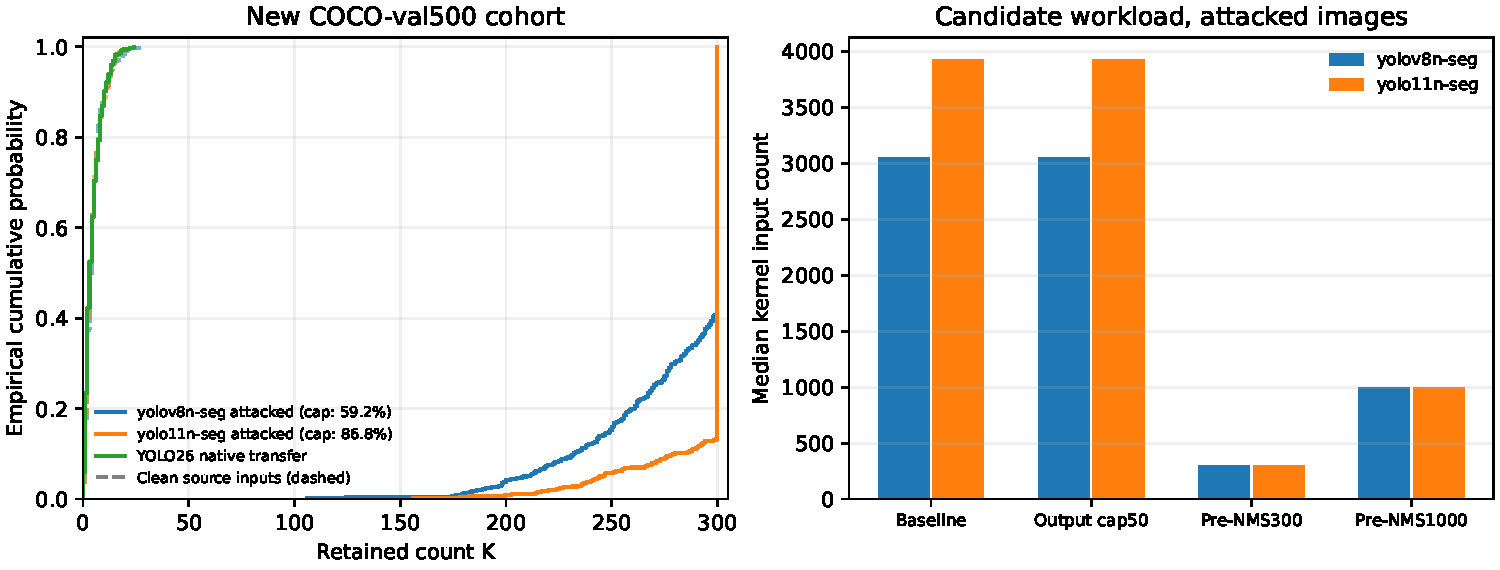
\includegraphics[width=0.95\textwidth]{segmentation_extension/val500_counts.pdf}\caption{Cohort COCO-val500 rời. Trái: phân bố số đếm thực nghiệm; đường nét đứt là đầu vào nguồn sạch, đường liền là đầu vào nguồn nhiễu hoặc chuyển native. Khối cuối ở $K=300$ là cap đầu ra. Phải: trung vị số ứng viên tới kernel NMS cố định. Số đếm khối lượng tự nó không thiết lập giảm độ trễ hay từ chối dịch vụ.}\label{fig:seg-val500}\end{figure*}
Nghiên cứu mở rộng gồm mọi kết quả ở bốn thiết lập cap và giữ mảng nhiễu float32, đầu ra native và hash. Đầu vào tấn công/đếm dùng resize vuông trực tiếp, còn đánh giá độ chính xác sạch riêng dùng letterbox; chúng không định nghĩa một đường accuracy--latency khớp chung. So sánh giữa mô hình nguồn là mô tả, không quy nhân quả cho kiến trúc. Đạt một ngưỡng đếm có thể gồm cả ảnh vốn đã trên ngưỡng khi sạch. Nghiên cứu đếm này không biến các phiên timing bị loại thành bằng chứng độ trễ hợp lệ và không thiết lập độ bền đặc thù mục tiêu của YOLO26.

\subsection{Nhận diện backend và timing pipeline thật}
Kiểm tra mã Ultralytics đã cài cho thấy dispatch phụ thuộc import: khi có torchvision trong \texttt{sys.modules}, wrapper gọi \texttt{torchvision.ops.nms}; nếu không, nó gọi \texttt{TorchNMS.nms}. Các script gốc khác nhau ở import này. Một so sánh kernel cùng-tensor tái lập sự chênh lệch, nhưng chẩn đoán đầy đủ đó trượt cổng trôi-tham-chiếu và được giữ như bằng chứng chẩn đoán chứ không phải một ước lượng độ trễ sạch để làm số chủ đạo. Phân biệt ở mức mã này loại trừ việc quy mức chậm lớn lịch sử cho riêng việc dựng mask.

\subsection{Độ chính xác dữ liệu sạch của các cap}
Toàn bộ 5.000 ảnh COCO val2017 được đánh giá bằng chỉ số phân đoạn nhãn-polygon của Ultralytics, không phải điểm COCO API tính lại độc lập. Suy luận dùng letterbox $640$ px, FP32, batch size 8, confidence 0.001, IoU 0.7 và workers 0. Ngưỡng confidence thấp hơn là thiết lập đánh giá độ chính xác cố định, khác ngưỡng tấn công. Đầu vào chỉ số mức detection được giữ để replay.
\begin{table*}[t]\centering
\caption{mAP50--95 phân đoạn trên toàn tập xác nhận và thay đổi tuyệt đối theo điểm phần trăm.}
\label{tab:seg-defense}
\begin{adjustbox}{max width=\textwidth}\begin{tabular}{llrr}\toprule Mô hình & Thiết lập & mAP (\%) & $\Delta$ (pp)\\\midrule
yolov8n-seg & Cơ sở & 30.23 & +0.00 \\
yolov8n-seg & Cap đầu ra 50 & 29.85 & -0.38 \\
yolov8n-seg & Cap trước NMS 300 & 30.01 & -0.22 \\
yolov8n-seg & Cap trước NMS 1000 & 30.22 & -0.01 \\
yolo11n-seg & Cơ sở & 31.88 & +0.00 \\
yolo11n-seg & Cap đầu ra 50 & 31.48 & -0.40 \\
yolo11n-seg & Cap trước NMS 300 & 31.64 & -0.25 \\
yolo11n-seg & Cap trước NMS 1000 & 31.88 & +0.00 \\
\bottomrule\end{tabular}\end{adjustbox}\end{table*}
Một cap đầu ra giới hạn số mask nhưng không chặn việc làm trước NMS. Một cap trước NMS giới hạn khối lượng ứng viên và có chi phí độ chính xác riêng. Các kết quả dữ liệu sạch này một mình không thiết lập độ bền chống tấn công hay tương đương thống kê. Không suy ra tuyên bố ý nghĩa nào từ chênh lệch mAP mô tả nhỏ. Một replay chỉ-đếm đăng ký riêng trên 20 đầu vào nhiễu đã khóa xác nhận phân biệt ranh giới: cap đầu ra 50 giữ nguyên số đầu vào kernel (1728--3744), còn cap trước NMS 300 giới hạn kernel về 300 ứng viên trên mọi ảnh. Trung vị số giữ lại sau cap trước NMS đó là 98; điều này không thiết lập việc loại bỏ chi phí mask hay một lợi ích độ trễ đo được.
\paragraph{Khả năng tái lập và giới hạn.} Các lần chạy thiết bị và đếm-native được đăng ký trước riêng, có một bổ sung head-native tường minh trước khi quan sát số đếm. Đánh giá độ chính xác được đăng ký trước riêng; các bổ sung chỉ-cài-đặt và lần smoke thất bại được giữ. Nghiên cứu bao một host/GPU thuê, các cohort timing/tấn công nhỏ cố định, các đối chứng khối lượng mask tổng hợp, và tấn công toàn ảnh dạng số. Nó không thiết lập từ chối dịch vụ ở camera hay thiết bị biên.

\subsection{Cohort lồng nhau và tấn công đặc thù mục tiêu trên mô hình không NMS}
\label{sec:nested1500}
Chúng tôi tính lại một cohort COCO-val lồng 1.000/1.500 ảnh với năm start mỗi ảnh và bốn đường tấn công (30.000 tấn công ảnh--start). Các tiền tố không phải tái lập độc lập. Mọi đường dùng 100 bước PGD, $\epsilon=16/255$, $\alpha=2/255$, đánh giá FP32 unfused, và iterate cuối. Một start không và bốn start ngẫu nhiên đều theo khóa-ảnh được cố định đón đầu. Hai mục tiêu đặc thù chia sẻ cùng nhiễu ban đầu cho mỗi ảnh và start.
\begin{table*}[t]\centering\small
\caption{Endpoint đếm của cohort lồng. K được trung bình trên năm start mỗi ảnh trước khi lấy trung vị. Reach là tỷ lệ ảnh--start trung bình; khoảng 95\% phân cấp lấy mẫu lại ảnh rồi start trong mỗi ảnh được lấy (20.000 lần). Đầu ra native dùng cột điểm 4 trên 0.25 và không NMS.}
\label{tab:nested1500}\begin{adjustbox}{max width=\textwidth}\begin{tabular}{rlrr}\hline
Ảnh & Mục tiêu/đánh giá & Trung vị K [95\% CI] & Reach $K\geq50$ (\%)\\\hline
1000 & v8/own & 289.40 [288.60, 292.20] & 100.00 [100.00, 100.00]\\
1000 & 11/own & 300.00 [300.00, 300.00] & 100.00 [100.00, 100.00]\\
1000 & v8/native26 & 3.00 [2.80, 3.40] & 0.00 [0.00, 0.00]\\
1000 & 11/native26 & 2.80 [2.60, 3.00] & 0.00 [0.00, 0.00]\\
1000 & 26-many/native26 & 287.60 [287.60, 291.90] & 99.98 [99.92, 100.00]\\
1000 & 26-native/native26 & 217.80 [215.30, 221.20] & 99.92 [99.78, 100.00]\\
1500 & v8/own & 289.40 [289.30, 292.20] & 100.00 [100.00, 100.00]\\
1500 & 11/own & 300.00 [300.00, 300.00] & 100.00 [100.00, 100.00]\\
1500 & v8/native26 & 3.20 [3.00, 3.40] & 0.00 [0.00, 0.00]\\
1500 & 11/native26 & 3.00 [2.80, 3.00] & 0.00 [0.00, 0.00]\\
1500 & 26-many/native26 & 287.80 [288.40, 292.00] & 99.97 [99.91, 100.00]\\
1500 & 26-native/native26 & 218.00 [216.40, 221.20] & 99.92 [99.81, 100.00]\\
\hline\end{tabular}\end{adjustbox}\end{table*}
Kết quả chuyển 0-trên-500 trước đó liên quan nhiễu tối ưu trên YOLOv8 và đánh giá trên head một-một native YOLO26. Nó không thiết lập miễn nhiễm với một tấn công đặc thù mục tiêu. Kiểm mã đã cài và một chẩn đoán bốn-ảnh đăng ký riêng tìm thấy gradient đầu vào hữu hạn, khác không cho cả hai head mục tiêu; đặc trưng backbone chỉ bị tách ở chế độ huấn luyện. Nghiên cứu lớn hơn phân biệt chuyển nguồn, tối ưu một-nhiều mục tiêu, và tối ưu điểm-native trong khi luôn đánh giá trực tiếp đầu ra native. Endpoint đếm chính là trung bình mức-ảnh qua các start, với bất định ảnh--start phân cấp. Khoảng Wilson mỗi start dùng số ảnh làm mẫu số. Thành công bất-kỳ-start là thứ cấp và tốn tới 500 bước gradient mỗi ảnh; nó không phải so sánh cùng chi phí với một start 100 bước. Ngưỡng chung native $K\geq50$ là ngưỡng đếm, không phải ngưỡng độ trễ đã thiết lập thực nghiệm cho YOLO26. Khoảng bootstrap thực nghiệm có thể co ở endpoint toàn-0 hoặc toàn-1; một khoảng biên như vậy không phải chắc chắn tổng thể, nên báo cận Wilson mỗi start thay thế. Khoảng percentile phân cấp đã đăng ký cho trung vị target-many 1.500 ảnh là [288.40, 292.00], trong khi ước lượng điểm là 287.8. Chúng tôi giữ sai lệch này thay vì sửa khoảng đã đăng ký sau khi thấy kết quả.
\begin{figure*}[t]\centering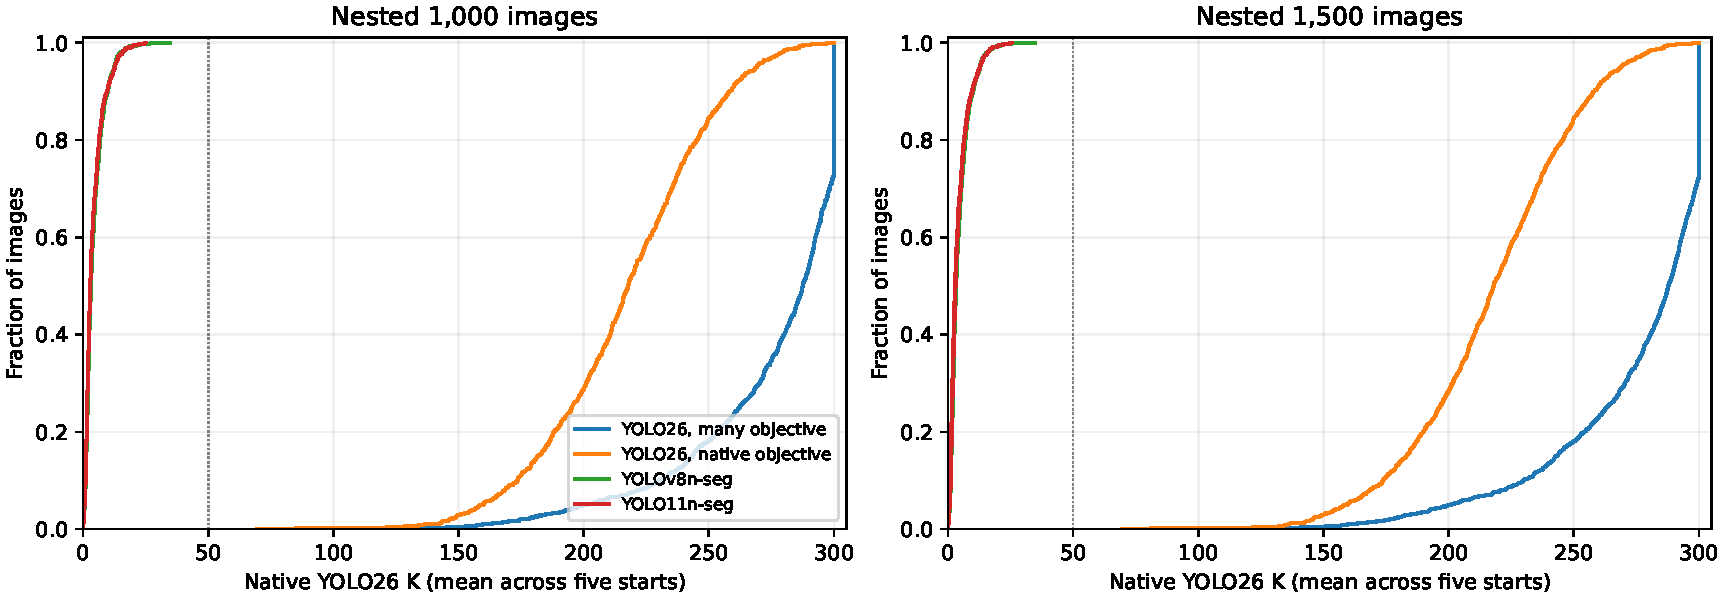
\includegraphics[width=\textwidth]{segmentation_extension/nested1500_native.pdf}\caption{Phân bố số đếm native YOLO26 dưới cả hai nguồn chuyển và cả hai mục tiêu đặc thù. Mỗi ảnh đóng góp trung bình số đếm trên năm start.}\label{fig:nested1500}\end{figure*}
Mọi trường hợp giữ vector điểm ứng viên, detection và đầu ra native. Đầu vào adversarial chính xác chỉ giữ cho tập audit 64 ảnh chọn đón đầu; các trường hợp còn lại có hash đầu vào và kiểm đầu-ra-đã-lưu, không replay đầu vào đầy đủ. Các kết quả đếm này không sửa được các cổng chất lượng timing đã trượt và không thiết lập một từ chối dịch vụ toàn trình.

\subsection{Đo lại laptop CPU với đầu vào nhiễu thật}
\label{app:seg-laptop}
Sau các chiến dịch timing bị loại trước đó, một audit mã phát hiện mất cân bằng carryover: các nhãn A/A trùng có vị trí tuyệt đối bằng nhau nhưng phân bố khối lượng sạch/nhiễu trước đó không bằng. Lời gọi cũng giữ lại đầu ra trước trong lần gọi kế. Một giao thức đón đầu mới cân bằng nhãn đồng thời theo khối lượng trước đó và vị trí cặp, dùng cùng callable cho cả hai nhãn, và giải phóng đầu ra sau khi cả hai đồng hồ dừng. Các thay đổi này là một gói; quan sát không cô lập cơ chế allocator, cache hay scheduler. Mọi thất bại trước vẫn bị loại. Hai phiên gắn tag đón đầu tái dùng cùng 20 cặp ảnh PGD toàn-ảnh đã khóa ($L_\infty=16/255$, 100 bước) và YOLOv8n-seg, với suy luận FP32 unfused, mask native $640\times640$, confidence 0.25, IoU 0.45 và backend NMS torchvision cố định. Worker laptop i5-1335U được ghim vào logical CPU 2, một hardware thread của một P-core, với một intra-op và một inter-op thread. Ưu tiên AboveNormal và HighQoS là process-local; cây ứng dụng trợ lý tạm tránh CPU 2 và SMT sibling 3 của nó, có khôi phục ghi nhật ký. Không đổi power-plan hay bảo vệ nhiệt.
\begin{table*}[t]\centering
\caption{Hai phiên có cổng riêng trên cùng 20 cặp ảnh đã khóa. Tỷ số là trung bình hình học của trung vị độ trễ toàn trình nhiễu/sạch theo ảnh. Cả hai phiên đạt; chúng không phải tái lập ảnh hay thiết bị độc lập.}
\label{tab:seg-laptop}
\begin{adjustbox}{max width=\textwidth}\begin{tabular}{lrrrr}\toprule
Phiên & Tỷ số toàn trình [95\% CI] & MDE A/A sạch (\%) & MDE A/A nhiễu (\%) & Số cờ trôi\\\midrule
1 & 4.235134 [4.024954, 4.441712] & 0.996622 & 0.213432 & 1/22 \\
2 & 4.222968 [4.007657, 4.433076] & 0.829358 & 0.168182 & 0/22 \\
\bottomrule\end{tabular}\end{adjustbox}\end{table*}
\begin{figure*}[t]\centering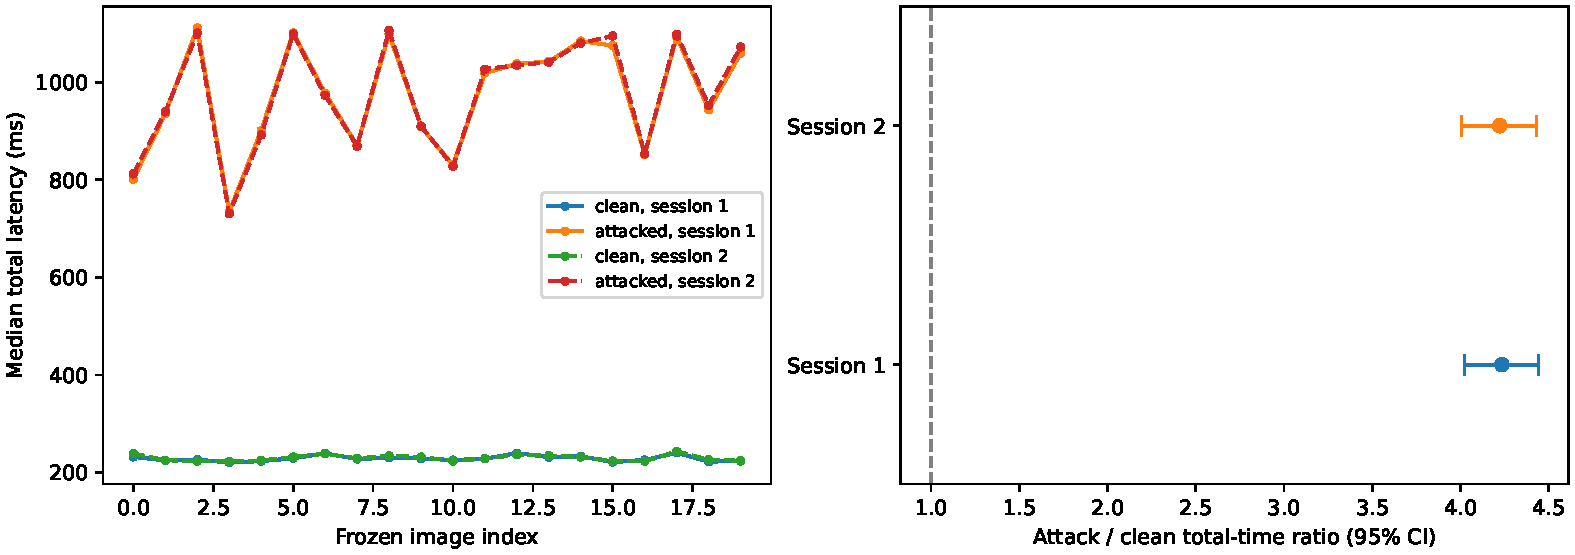
\includegraphics[width=.9\textwidth]{segmentation_extension/laptop_sessions.pdf}\caption{Trung vị độ trễ theo ảnh đã lưu và các khoảng tỷ số của từng phiên riêng. Cùng ảnh và lịch tất định được chia sẻ; không dựng khoảng gộp liên-phiên.}\label{fig:seg-laptop}\end{figure*}
MDE sạch phiên đầu gần cổng 1\%; giá trị không làm tròn được dùng để xét điều kiện. Qua cổng dựa-trung-vị này không thiết lập độ trễ đuôi ổn định. Phiên 1 giữ 24/1920 lời gọi sạch và 42/1920 lời gọi nhiễu vượt 1.5 lần trung vị riêng của ảnh; phiên 2 giữ 14/1920 và 52/1920. Mỗi spike có process-CPU/wall dưới 0.75. Nguyên nhân chưa rõ. Phiên thứ hai được đăng ký sau khi xem phiên đầu và tái dùng cấu hình mà không tìm thêm lần lặp hay core. Các ước lượng tương tự là bằng chứng lặp lại mô tả, không phải kiểm tương đương. Không phiên nào cô lập NMS khỏi mask vì profiling từng-công-đoạn bị bỏ khỏi lịch chỉ-toàn-trình đã sửa này. Kết quả này ủng hộ chi phí tính toán tăng trên tensor chuẩn bị sẵn trong hai phiên trên một laptop và một mô hình. Nó không thiết lập từ chối dịch vụ, lỡ hạn chót, độ bền camera, hiệu quả patch phổ quát/cục bộ, hành vi ARM/Pi, hay tính hợp lệ timing cho cohort đếm 1500 ảnh riêng.

\subsection{Timing phòng thủ trước NMS (ghép cặp)}
\label{app:seg-laptop-defense}
Sau hai phiên CPU được chấp nhận, một giao thức đón đầu riêng cố định hai can thiệp: cap ứng viên trước NMS ở 300, hoặc cap đầu ra giữ lại ở 50. Mỗi so sánh dùng cùng tensor nhiễu đã khóa ở cả hai nhánh và một baseline xen kẽ đo mới (cap ứng viên 30000, cap đầu ra 300). Thiết bị, mô hình, backend NMS cố định, độ phân giải và lịch nhãn-trùng cân bằng carryover theo phương pháp laptop trên. Mỗi khối có smoke và full có điều kiện riêng, cổng chất lượng độc lập, khóa nguồn/đầu-vào SHA và khôi phục affinity ứng dụng. Một probe tạm ghi số đầu vào kernel biên dịch thật ngoài vùng timing và khôi phục hàm gốc trước warmup và đo.
\begin{table*}[t]\centering
\caption{Các so sánh phòng thủ đặt trước. Chỉ can thiệp trước-NMS đạt đủ điều kiện timing. Lần smoke cap-đầu-ra thất bại được giữ và full bị hủy, không chạy lại.}
\label{tab:seg-laptop-defense}
\begin{adjustbox}{max width=\textwidth}\begin{tabular}{lrrrr}\toprule
Can thiệp & Phòng thủ/baseline [95\% CI] & MDE A/A baseline (\%) & MDE A/A phòng thủ (\%) & Số cờ trôi\\\midrule
Cap trước NMS 300 & 0.526773 [0.507007, 0.548921] & 0.149061 & 0.314700 & 1/22 \\
Cap đầu ra 50 & Không đạt; full bị hủy & --- & --- & 1/4 (smoke) \\
\bottomrule\end{tabular}\end{adjustbox}\end{table*}
Với cap trước NMS, độ trễ toàn trình giảm 47.322709\% [95\% CI theo điểm 45.107882, 49.299341]. Chênh lệch trung bình ghép cặp của trung vị theo ảnh là -468.920147 ms [95\% CI -510.113507, -425.613187]. Mỗi khoảng dùng 20000 lần bootstrap-ảnh đã đăng ký; các khoảng này không phải khoảng đồng thời theo họ. Cả 20 log tỷ số theo ảnh cùng dấu âm. Kiểm đảo dấu chính xác hai phía duyệt toàn bộ $2^{20}$ phép gán, cho $p=2/2^{20}$; hiệu chỉnh Holm trên hai so sánh đã đăng ký cho $p_{\mathrm{Holm}}=4/2^{20}$. So sánh cap-đầu-ra chưa đo/thất bại đóng góp một placeholder kiểm định bằng một để giữ cỡ họ; giá trị đó không phải phát hiện không hiệu ứng. Số đầu vào kernel quan sát được giảm từ 1726--3744 xuống đúng 300 cho mọi ảnh. Mask giữ lại đổi từ trung vị 270.5 (khoảng 177--300) xuống 98 (84--118). Vậy can thiệp chặn đầu vào kernel nhưng vẫn giữ việc mask khác không; tương phản toàn-trình này không quy riêng tiết kiệm cho NMS và dựng mask.
\begin{figure*}[t]\centering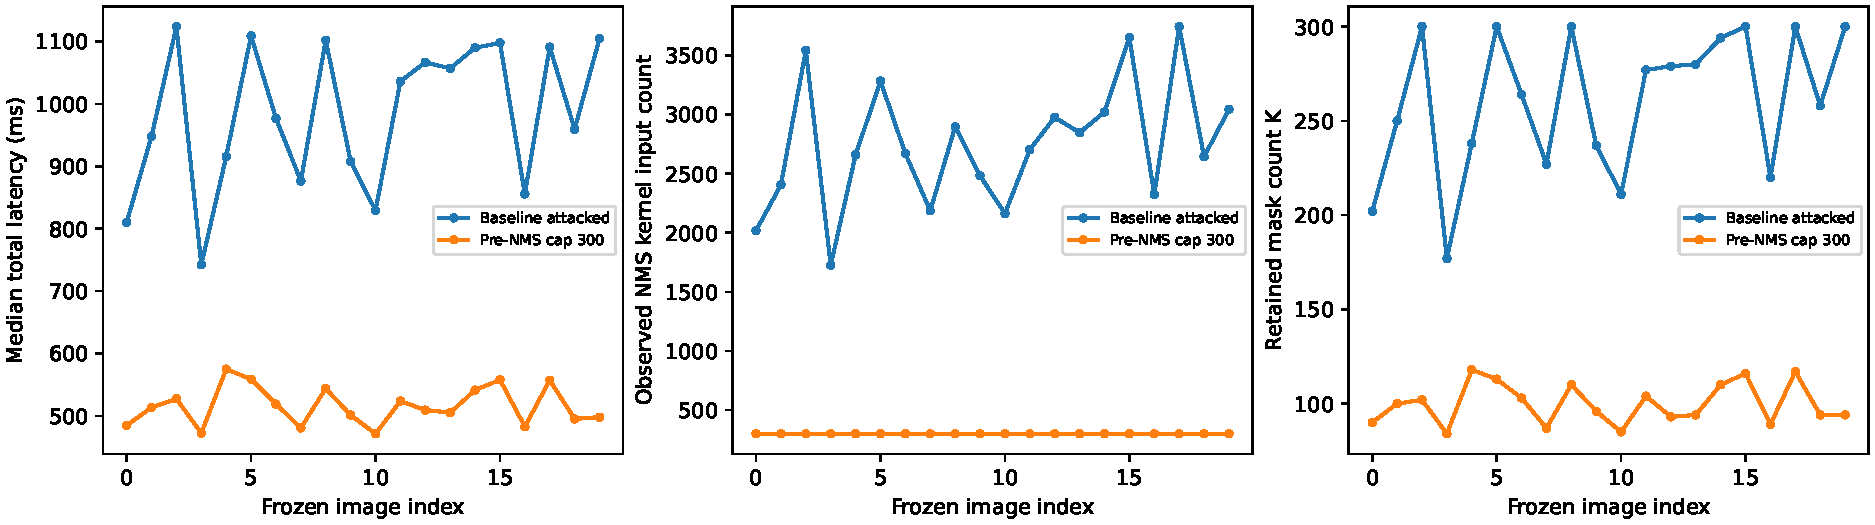
\includegraphics[width=.98\textwidth]{segmentation_extension/laptop_defense.pdf}\caption{Can thiệp trước-NMS đạt chất lượng: trung vị độ trễ toàn trình theo ảnh, số đầu vào NMS biên dịch quan sát được, và số mask giữ lại. Số đếm và timing có trục và đơn vị riêng.}\label{fig:seg-laptop-defense}\end{figure*}
Lần smoke cap-đầu-ra có tỷ số tham chiếu forward 1.0376 ở ảnh đầu, vượt cận 3\% đã đăng ký; các timing thấp hơn bề ngoài của nó giữ là chẩn đoán và không dùng như ước lượng phòng thủ đạt chất lượng. Nghiên cứu kiểm nhiễu đã lưu cố định, không phải một đối thủ thích ứng huấn luyện chống cap.

\subsection{Raspberry Pi vật lý: phiên toàn-cohort đạt thời gian toàn trình, trượt độ chính xác công đoạn}
\label{app:seg-pi3b-full20}
Sau khi xem pilot bị loại, một giao thức đăng ký riêng đã duyệt chạy cohort 20 ảnh theo kế hoạch ban đầu một lần, không pilot thêm hay nới cổng toàn-cohort. Nó tái dùng cùng nhiễu và ảnh đã khóa; không phải cohort độc lập hay tái lập chọn trước mọi quan sát Pi. Thực thi bốn luồng ghim vào bốn CPU Cortex-A53, với suy luận FP32 và mask native toàn độ phân giải. Điều kiện nguồn đã khai báo và governor powersave được giữ; xung lấy mẫu là 600~MHz, với cả cờ under-voltage hiện-tại-cộng-lịch-sử lẫn chỉ-lịch-sử. Không quy đổi sang performance ở xung khác. Pipeline chính hoàn tất 720 lần đo. Cả hai kiểm tải đạt, 0/22 điểm tham chiếu bị cờ, và mọi guard điều kiện ghi nhật ký đạt với swap tắt. Tỷ số A/A hình học là 0.9990 và log-MDE công suất 80\% theo ảnh là 0.00275, dưới 0.05. Khôi phục cấu hình độc lập cũng đạt. Các tỷ số thời gian toàn trình chính do đó đạt chất lượng dưới giao thức này: nhiễu/sạch là 1.798 [95\% CI 1.747, 1.848], và cap-ứng-viên/nhiễu là 0.729 [0.713, 0.746]. Cả hai kiểm đảo dấu chính xác hai phía có $p$ thô $0.00000191$ và $p$ Holm $0.00000381$ trong họ chính hai-giả-thuyết. Khoảng lấy mẫu lại ảnh 20.000 lần; chúng không phủ biến thiên theo seed-nhiễu, board hay nguồn. Trung vị tỷ trọng forward theo ảnh là 98.6\% cho đầu vào sạch và 54.0\% cho đầu vào nhiễu. Phiên công đoạn kế hoàn tất 705 lần đo trên cả 20 ảnh, gồm các liều đếm-mask trên năm ảnh đầu. Tuy nhiên tỷ số A/A hình học NMS khối-lượng-nhiễu là 0.9476, với log-MDE 0.1652: cả hai cổng độ chính xác NMS trượt. Đối chứng mask tương ứng là 0.9941, với log-MDE 0.0271, đạt cổng riêng. Cổng công đoạn ghép đã đăng ký vẫn trượt: mọi ước lượng công đoạn và liều giữ là chẩn đoán, và phiên một-luồng chưa khởi chạy bị hủy. Không ảnh nào bị bỏ và không phiên nào chạy lại. Cả 20 cặp khớp số ứng viên và số mask giữ lại của laptop, nhưng 0/40 tensor dự đoán sạch/nhiễu khớp từng byte. Phiên bản PyTorch/torchvision khác nhau. Phát lại thời gian toàn trình đạt này không lật lại hai giao thức bị loại trước, không thiết lập lỗi hạn chót dịch vụ hay từ chối dịch vụ, hay xác nhận một patch vật lý hay thiết bị khác.

\subsection{Raspberry Pi vật lý: một luồng với SSD USB nằm im}
\label{app:pi3b-pi1}
Một lần chạy đăng ký riêng đo cùng hai mươi cặp đã khóa và YOLOv8n-seg trên một lõi CPU ghim của cùng board, ở cùng điều kiện 600~MHz do under-voltage đã khai báo. Khác lần bốn luồng, một SSD USB cấp nguồn riêng (ADATA SP900, chưa mount) được cắm suốt; đây là \emph{một điều kiện khai báo riêng} và không gộp với kết quả bốn luồng. Lần chạy ghi bộ đếm I/O khối SSD ở mỗi lần chụp môi trường: số sector ghi giữ ở không trên cả hai ổ USB suốt phiên, nên ổ được xác minh nằm im lúc timing. Phiên đạt mọi cổng chất lượng, gồm cổng ổ-nằm-im, với swap tắt, xung khóa 600~MHz, 0 tham chiếu bị cờ và sàn nhiễu A/A ứng với MDE 1.002. Trên một lõi, tỷ số độ trễ toàn trình nhiễu/sạch là 1.967 (95\% CI [1.902, 2.030]; cả 20 ảnh dương), lớn hơn tỷ số bốn luồng vì dựng mask hưởng lợi từ nhiều luồng trong khi việc mask nhiễu chi phối trên một lõi. Một cap trước NMS kéo toàn trình nhiễu còn một hệ số 0.699 (95\% CI [0.682, 0.718]). Trung vị độ trễ toàn trình là 10.05~s sạch, 20.30~s nhiễu và 13.77~s cap; forward chiếm 99\% toàn trình sạch. Các số một-lõi này mô tả một board thiếu áp với một thiết bị USB nằm im khai báo và không chuyển sang điểm làm việc 1.2~GHz, sang điều kiện không-USB, hay sang từ chối dịch vụ.

\subsection{Một can thiệp bộ nhớ renderer trên Pi (riêng)}
\label{app:seg-pi3b-memory}
Một giao thức về sau, đăng ký trước quan sát bộ nhớ đầu tiên, so renderer native đã khóa (ngân sách chunk 32 triệu pixel) với một cài đặt kết hợp cấp-phát-trước đầu ra uint8/chép-trực-tiếp dùng ngân sách 16 triệu pixel. Nhân hệ số, resize, ngưỡng và crop được giữ. So sánh tái dùng cùng 20 cặp đầu vào sạch/nhiễu đã quan sát, một khởi tạo tấn công mỗi ảnh. Pi 3B vật lý vẫn bị under-voltage giới hạn ở 600~MHz với bốn luồng. Một SSD cắm chủ đích, chưa mount và nằm im; đường source/cache/log vẫn trên thẻ SD. Đây là điều kiện khai báo riêng chứ không phải chạy lại lần smoke bộ nhớ không-USB trước (vốn abort ở guard USB trước mọi mẫu RSS; lần smoke thất bại đó và full bị hủy được giữ). Mỗi tiến trình mới import runtime, kiểm một cache đã khóa, warmup một mask cùng-renderer, render và hash đầu ra. Không mô hình nào thường trú trong tiến trình đó. \texttt{ru\_maxrss} Linux được đọc sau digest và đổi từ KiB sang byte. Endpoint gồm import, kiểm, warmup, observer, allocator/workspace và đầu ra; nó không phải đỉnh bộ nhớ renderer riêng. Cả hai bản native (A/B) và candidate, mỗi cái lặp ba lần cho cả sạch/nhiễu, được ngẫu nhiên hóa trong mỗi ảnh/lần lặp. Mẫu số theo ảnh gộp cả sáu mẫu native trước khi lấy trung vị; tử số là trung vị ba mẫu candidate. Ảnh, không phải tiến trình, là đơn vị suy luận. Cả 360 tiến trình mới hoàn tất và mọi digest đầu ra khớp digest cache đã khóa. Cả đối chứng A/A sạch và nhiễu đạt cận log-tỷ-số-trung-bình tuyệt đối cố định 0.02 và cận MDE 0.05; MDE của chúng là 0.00010053 và 0.00007975. Với endpoint xác nhận nhiễu duy nhất, tỷ số đỉnh-toàn-tiến-trình candidate/native hình học là 0.875504 (95\% CI bootstrap-ảnh [0.867516, 0.883885]), thấp hơn khoảng 12.45\%. Bootstrap 20.000 lần dùng seed 2026111401; giá trị đảo dấu hai phía chính xác là $2/2^{20}=0.000001907349$, độ phân giải nhỏ nhất, với mọi đơn vị ảnh cùng chiều. Cỡ hiệu ứng log-tỷ-số ghép cặp là $d_z=-5.9763$. Kết quả trường hợp sạch là mô tả: tỷ số 0.996475, CI [0.995843, 0.997081]. Thay đổi kết hợp không cô lập tác động của cỡ chunk và dựng đầu ra. Nó thiết lập một mức giảm bộ nhớ có điều kiện trên các cache này và thiết bị/runtime này; không cung cấp RSS mô-hình-thường-trú tích hợp, độ trễ renderer, thông lượng, năng lượng, ước lượng độ chính xác mới hay lỗi hạn chót. RSS giảm một mình không xác định nguyên nhân biến thiên NMS hay thiết lập từ chối dịch vụ.

\subsection{Kết quả âm và các đối chứng bị loại}
Để minh bạch, các kiểm soát sau được thực hiện nhưng \emph{không đạt} cổng chất lượng đã đăng ký và chỉ giữ như bằng chứng chẩn đoán trong kho mã, không dùng làm số liệu: (i) các đối chứng công đoạn chuẩn-bị-sẵn trên laptop (NMS và mask dựng riêng) trượt cổng trôi-tham-chiếu (20/22 khối bị cờ ở NMS; smoke mask bị cờ); (ii) một chẩn đoán chỉ-forward (không NMP/mask) vẫn thấy trôi tham chiếu vượt 3\%, nên trôi không do riêng NMS hay mask; (iii) một smoke ghim hai P-core bị loại vì 2/4 tham chiếu bị cờ; (iv) lần phát lại Pi đầu tiên hoàn tất 720 lần đo nhưng swap tự bật lại giữa chừng, vi phạm điều kiện swap-tắt; (v) một pilot Pi có khóa swap về sau trượt độ chính xác (log-MDE 0.1335 trên hai ảnh). Mọi lần thất bại giữ nguyên trạng thái bị loại; không lần nào được chạy lại để lấy số đẹp, và không phần nào ở trên bị loại làm mất hiệu lực các phiên đạt chất lượng.
